% vim: set tw=78 sts=2 sw=2 ts=8 aw et:
\documentclass{so.cs.pub.ro}

%\usepackage{code/highlight}

\title[Laborator 10]{Laborator 10}
\subtitle{Operaţii I/O avansate - Windows}

\begin{document}

\frame{\titlepage}


% NB: Secțiunile nu sunt marcate vizual, ci doar apar în cuprins

% Titlul unui frame se specifică fie în acolade, imediat după \begin{frame},
% fie folosind \frametitle
\begin{frame}{Modele de operaţii I/O}
\begin{columns}
  \begin{column}[1]{0.55\textwidth}
    \framebox{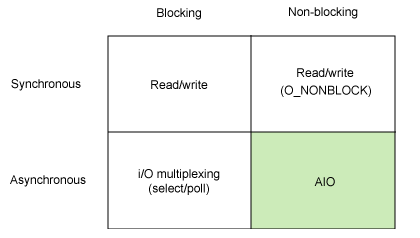
\includegraphics[height=1.3in]{code/ioModel.png}}
  \end{column}
  \begin{column}[1]{0.45\textwidth}
    \begin{itemize}    % Just like normal LaTeX
    \item Operaţii blocante
    \begin{itemize}
        \item Wait
     \end{itemize}
    \item Operaţii non-blocante
    \begin{itemize}
	\item Don't wait
    \end{itemize}
\vspace*{0.2cm}
    \item Notificare
    \begin{itemize}
	\item Sincron
	\item Asincron
    \end{itemize}
    \end{itemize}
  \end{column}
\end{columns}
\end{frame}

\begin{frame}{Operaţii asincrone în Windows}
  \begin{itemize}    % Just like normal LaTeX
    \item \textbf{Overlapped I/O}
\vspace*{0.2cm}
    \item File handle creat cu flag-ul FILE_FLAG_OVERLAPPED
\vspace*{0.2cm}
    \item Structura OVERLAPPED folosită de ReadFile, WriteFile
	\begin{itemize}
	\item Codul de eroare pentru cererea I/O
	\item Numărul de octeţi transferaţi
	\item Poziţia în fişier de unde se face operaţia I/O
	\item Un eveniment care va fi semnalizat când operaţia se termină
        \end{itemize}
\vspace*{0.2cm}
    \item GetOverlappedResult
	\begin{itemize}
	\item Obţine rezultatul unei operaţii I/O overlapped
	\end{itemize}
  \end{itemize}
\end{frame}

\begin{frame}{Completion Ports}
  \begin{itemize}    % Just like normal LaTeX
    \item Obiect în kernel care asociază un set de overlapped handles cu un set de fire de execuţie
    \item Firele de execuţie aşteaptă ca operaţiile de I/O să se încheie
  \end{itemize}
\begin{columns}
  \begin{column}[1]{0.48\textwidth}
  \center{\framebox{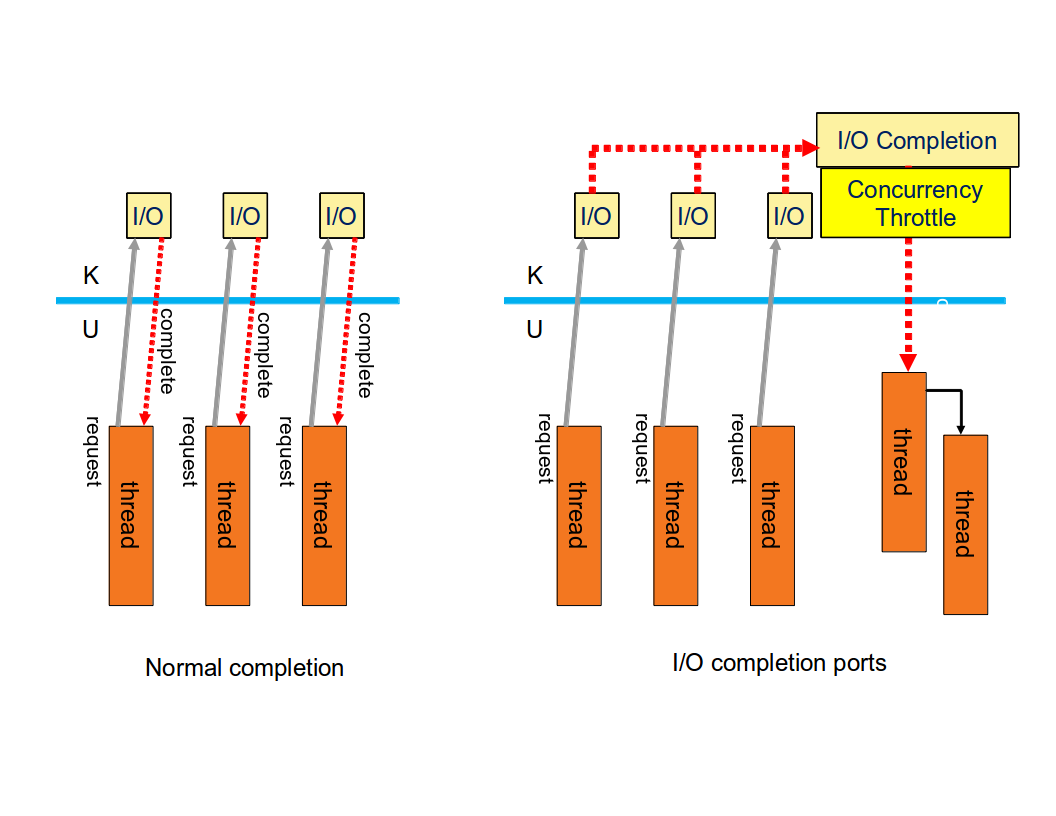
\includegraphics[height=1.6in]{code/ioCompletion.png}}}
  \end{column}
  \begin{column}[1]{0.52\textwidth}
  \begin{itemize}
    \item CreateIoCompletionPort
    \item GetQueuedCompletionStatus
  \end{itemize}
  \end{column}
\end{columns}
\end{frame}

\begin{frame}{Zero Copy I/O}
  \begin{itemize}    % Just like normal LaTeX
    \item Evită copierea datelor dintr-o zonă într-alta
    \item TransmitFile - transmite un fişier peste un socket
  \end{itemize}
\begin{columns}
  \begin{column}[1]{0.5\textwidth}
  \center{\framebox{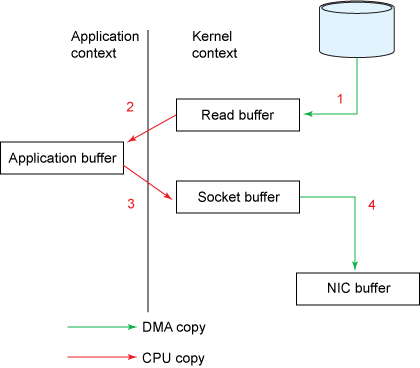
\includegraphics[height=2in]{code/normalCopy.png}}}
  \end{column}
  \begin{column}[1]{0.5\textwidth}
  \center{\framebox{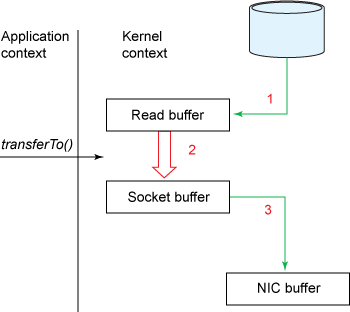
\includegraphics[height=2in]{code/zeroCopy.png}}}
  \end{column}
\end{columns}
\end{frame}

%\begin{frame}{Întrebări}
%\begin{itemize}
%\item Ce mecanism aţi folosi pentru tratarea operaţiilor cu placa de reţea: polling sau întreruperi?
%\item De ce sunt operaţiile cu dispozitivele de I/O asincrone?
%\item Fac parte registrele de I/O din contextul unui proces?
%\item Are sens folosirea operaţiilor de tipul overlapped I/O pe un sistem cu un singur hard-disk?
%\end{itemize}
%\end{frame}

\end{document}
